\documentclass[12pt, a4paper]{article}
\usepackage[utf8]{inputenc}

% Format
\usepackage{layout}
\setlength{\parindent}{0.5in}
\setcounter{secnumdepth}{0}
\usepackage{lineno}

% Font
\usepackage{MinionPro}
\input glyphtounicode
\pdfgentounicode=1
\usepackage{microtype}
\usepackage[super]{nth}
\usepackage{tfrupee}

% Language
\usepackage[british]{babel}

% References
\usepackage[nosectionbib, tocbib, unnumberedbib]{apacite}

% Figures
\usepackage{graphicx}
\usepackage[small, labelfont=it, labelsep=period]{caption}

% Tables
\usepackage{booktabs}
\usepackage{tabularx}

% Commands
\newcommand{\pest}[4]{$ \text{Pr} (\text{``us''} | \text{#1}) = #2$, $[#3, #4]$}
\newcommand{\pdif}[4]{$ \Delta\text{Pr} (\text{``us''} | \text{#1}) = #2$, $[#3, #4]$}

% Frontmatter
\title{Intergroup contact fosters\\more inclusive social identities}
\date{August 23, 2018}


\begin{document}

\maketitle

\begin{abstract}
\noindent We examined how South Indian students construct their social identities from multiple group memberships---and whether contact with caste and religious outgroups fosters more inclusive social identities. Participants ($N = 351$) viewed 24 identity cards, each representing a person with whom participants shared none, one, two, or all three group memberships. Participants reported whether they considered each person as ``us'' or ``not us'', showing whom they included in their ingroup, and whom they excluded. Using this method, we found that participants tended to exclude caste and religious minorities, replicating persistent social divides. Bridging these divides, cross-group friendship was associated with more inclusive identities, while more inclusive identities were associated with more favourable outgroup attitudes. Negative contact---but not social dominance orientation---was associated with less inclusive identities, showing that past experiences shaped whom participants considered ``us'' and ``not us''. Contact and identity processes were unrelated to support for affirmative action.\\[1ex]
\noindent \textbf{Keywords:} \ldots\\[1ex]
\end{abstract}

\linenumbers

\noindent How we feel about and act toward other people depends on whom we consider ``us'' and ``them''---that is, whom we include in our ingroup, and whom we exclude (for a review, see Reimer, Schmid, Hewstone, \& Al Ramiah, in press). In some situations, it is clear who is in the ingroup and who is not. On a football pitch, for example, players tend to think of their own team as ``us'', and of the other team as ``them'', and try their best to make sure their own team wins. In many situations, this distinction is less clear because it rests on multiple category memberships. Often, the relevant categories are interrelated. Many Americans, for example, associate being American with being White American (Devos \& Banaji, 2005). This suggests that whom Americans consider ``us'' and ``them'' might depend on someone's race \emph{and} nationality (and perhaps other categories, such as religion or language). In this paper, we examine how people's group memberships shape whom they consider ``us'' and ``not us'', and test what the antecedents and consequences of more inclusive social identities are.

Social psychological theories have argued for the importance of two (Berry, 1997; Crisp \& Hewstone, 2007; Dovidio, Gaertner \& Saguy, 2009) or more (Roccas \& Brewer, 2002) social categories for understanding intergroup relations. Broadly, these perspectives recognise that we are part of multiple overlapping groups; that we have a subjective sense of who is ``us'' and ``them'' that goes beyond the objective facts of group membership; and that this identification across multiple categories affects our attitudes toward people with whom we share some, but not all, group memberships. However, these perspectives have lacked a method for measuring social identification across multiple overlapping categories.

Addressing this shortcoming, van Dommelen, Schmid, Hewstone, Gonsalkorale, and Brewer (2015) developed the triple crossed-categorization task to measure how individuals construct their social identities from multiple group memberships. In this task, participants view identity cards, each of which represents a fictitious person with whom participants share none, one, two, or all of three group memberships. Participants report whether they consider each person as ``us'' or ``not us'', showing whom they included in their ingroup, and whom they excluded. The researchers analysed participants' responses quantitatively, as social identity inclusiveness, and qualitatively, as social identity structure. They operationalised inclusiveness as the total number of targets a participant had categorized as ``us''. They coded response patterns according to structures proposed by Roccas and Brewer (2002). Figure~\ref{fig:f1} shows schematic representations of various plausible structures, ordered by their inclusiveness.

\begin{figure}
\centering
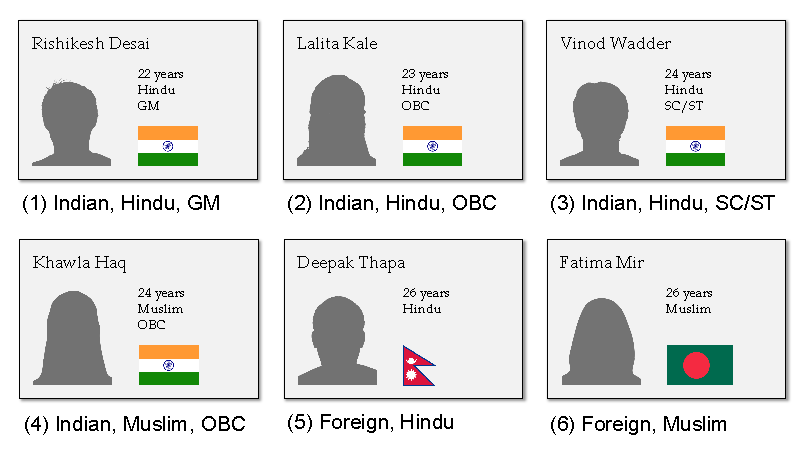
\includegraphics[scale=1]{../figures/figure-1}
\caption{
Schematic representations of social identity structures, ordered by social identity inclusiveness. Shaded regions represent the groups which a participant has to categorize as ``us'' to be assigned that structure. An Indian Hindu, for example, may consider only people who share their nationality, religion, and caste as ingroup members (intersection). Someone else may consider all their fellow Indians, whatever their religion or caste, as ingroup members (dominance). Another person may consider anyone who shares their nationality or religion as ingroup members (merger). % This person has a more inclusive social identity than the other two people.
}
\label{fig:f1}
\end{figure}

In two studies, van Dommelen et al. (2015) studied social identification across ethnicity, religion, and nationality among Turkish-Belgian Muslims and Turkish-Australian Muslims. Participants categorized, on average, 59\% and 65\% of targets as ``us'', and endorsed a wide range of social identity structures. As the researchers recruited homogeneous samples, they studied individual differences, but not group differences, in social identity inclusiveness. Participants' group memberships, however, likely influence whom they consider ``us'' and ``not us''. For majority-group members, negotiating their ethnic and national identities likely means something different that for minority-group members (Dovidio et al., 2009). As group members share these experiences, we expect that group differences are as great as, if not greater than, individual differences in social identity construals---especially if groups differ in status and power.

Shared experiences, however, make only part of an individual's day-to-day experiences. Of these, contact experiences could overcome group differences in social identity construals. First, encountering diverse others could initiate a process of cognitive differentiation (Schmid \& Hewstone, 2011) whereby interaction partners become aware of the complex interrelations of their cross-cutting group memberships. Second, intergroup interactions can motivate people to include the outgroup of an interaction partner in their self-concept (Page-Gould et al., 2010). As far as contact motivates people to include (partial) outgroups in the self, it should encourage social identities that include the inter-action partner's combination of group memberships. Together, these mechanisms suggest that intergroup contact could overcome group differences, and foster more inclusive social identities.

Fostering more inclusive identities could reduce intergroup bias. Dividing others into “us'' and ``not us'' is a necessary and sufficient condition for in-group favouritism (Tajfel, 1981). Considering more people as ``us'' should ex-tend ingroup favouritism to a wider range of people, and thus reduce discrimination (Gaertner et al., 2016). Ingroup favouritism can turn into outgroup derogation when an outgroup threatens the ingroup (Brewer, 1999). Considering fewer people as ``not us'' should reduce the number of groups which are perceived to threaten the ingroup. Together, these mechanisms suggest that more inclusive identities could reduce intergroup bias.

Beyond prejudice, researchers have debated whether fostering more inclusive identities helps or hinders social change. Changing attitudes and beliefs is often not enough to overcome structural inequalities. Instead, social change requires advantaged and disadvantaged groups to strive for redistributive policies. On the one hand, fostering more inclusive identities could break down the boundaries between the advantaged ingroup and the disadvantaged out-group---making injustice faced by ``them'' into ``our'' problem. This process could narrow the gap between advantaged-group members' support for the principle of equality and their opposition to its implementation in policies (Dixon, Durrheim \& Tredoux, 2007). On the other hand, fostering more inclusive identities could distract disadvantaged-group members from differences in resources and power, and thus reduce their support for social change (Dovidio, Saguy, Gaertner, \& Thomas, 2012). Together, these mechanisms suggest that more inclusive identities could increase support for social change among the advantaged, but decrease support among the disadvantaged.

\section{Present research}

In the present research, we examined how South Indian students construct their social identities from the overlapping categories of caste, religion, and nationality. Caste is a system of social relations that concentrates status and power in the hands of dominant castes (Jodhka, 2012). This system is maintained by restricting subordinate castes' occupations, by barring subordinate castes from owning land, and by enforcing endogamy and segregation. This system is underpinned by a tradition that ranks castes according to their supposed ritual purity, and condemns contact with less pure castes as polluting. Untouchability excludes some castes from public life, and consigns them to landlessness and menial labour. Dalits---members of castes that have been affected by untouchability---still face economic inequalities based on this history of exploitation, as well as interpersonal discrimination based on the practice of untouchability. Since Independence, the Indian State has sought to redress caste-based injustices by reserving seats in state-run universities and state-sector jobs for disadvantaged groups. Specifically, the Indian State recognises Dalits as Scheduled Castes (SCs), Adivasi---India’s indigenous peoples---as Scheduled Tribes (STs), and other disadvantaged castes (who fall above the so-called `line of pollution') as Other Backward Classes (OBCs). Members of historically advantaged castes compete for these opportunities in the General Merit (GM) category. Reservation policies, alongside ongoing discrimination, have resulted in caste identities remaining important in electoral politics and political organising.

\section{Method}

\begin{table}    
\caption[Participants by gender, age, nationality, religion, and caste]{Participants by gender, age, nationality, religion, and caste. Categories in \textit{italics} were excluded from the final sample. N/A marks missing responses.}
\centering
\figureversion{lining, tabular}
\small	
\begin{tabular}{llrr} \addlinespace \toprule
\multicolumn{2}{l}{Category} & $n$ & \% \\ \midrule \addlinespace 
Gender      & Woman      & 215 & 61 \\
            & Man & 121 & 34 \\
            & Other & 0 & 0 \\
            & N/A & 15 & 4 \\ \addlinespace \addlinespace
Age         & 18--20 & 1 & 0 \\
            & 21--23 & 254 & 72 \\
            & 24--26 &  77 & 22 \\
            & 27--29 &  10 &  3 \\
            & 30--32 &   1 &  0 \\
            & 33--35 &   0 &  0 \\
            & 36 or older & 1 & 0 \\ 
            & N/A & 7 & 2 \\ \addlinespace \addlinespace
Nationality & Indian & 339 & 97 \\
            & Other & 0 & 0 \\
            & N/A & 12 & 3 \\ \addlinespace \addlinespace
Religion    & Buddhism & 1 & 0 \\ 
            & Christianity & 11 & 3 \\ 
            & Hinduism & 297 & 85 \\ 
            & \textit{Islam} & \textit{27} & \textit{8} \\ 
            & Jainism & 8 & 2 \\ 
            & Other & 2 & 1 \\ 
            & N/A & 5 & 1 \\ \addlinespace \addlinespace
Caste       & General Caste & 104 & 30 \\ 
            & Other Backward Class & 143 & 41 \\ 
            & Scheduled Caste & 54 & 15 \\ 
            & Scheduled Tribe & 23 & 7 \\ 
            & \textit{Other / Not applicable} & \textit{20} & \textit{6} \\ 
            & \textit{N/A} & \textit{7} & \textit{2} \\ \addlinespace \midrule
Total       &   & 351 & 100 \\ \bottomrule
\end{tabular}
\label{tab:t1}
\end{table}

\begin{figure}
\centering
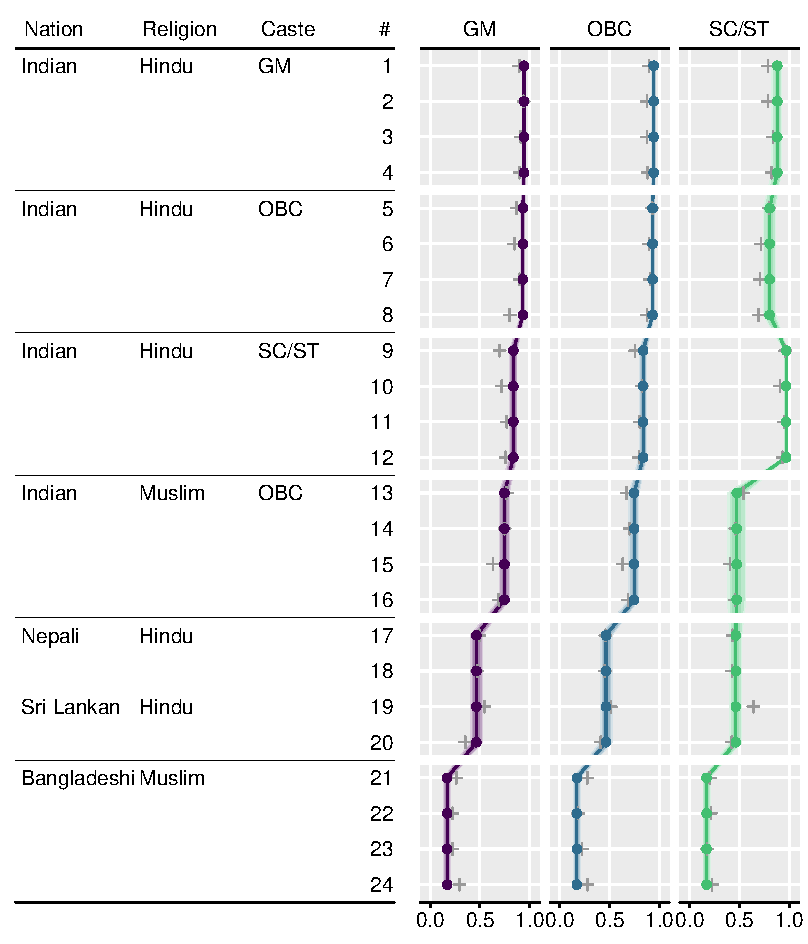
\includegraphics[scale=1]{../figures/figure-2}
\caption{Examples of targets used in the triple crossed-categorization task. Based on ratings in a pilot study ($N = 26$), we selected the four most prototypical targets (out of fifty initial targets) for each of six plausible combinations of caste, religion, and nationality (for details, see Appendix~A). Each target showed a person's caste (GM = General Merit, OBC = Other Backward Class, SC/ST = Scheduled Caste/Scheduled Tribe), religion (Hindu, Muslim), and nationality (Indian, Nepali, Sri Lankan, Bangladeshi). Each target also showed the person's first and last name, age (21--26 years), and a silhouette corresponding to the person's gender (adapted from Ma, Correll \& Wittenbrink, 2015). Each target's age and silhouette, as well as the order in which the targets were presented, varied across sessions.}
\label{fig:f2}
\end{figure}

\section{Results}

\begin{table}
\caption{
Comparison of models estimating the probability of participants categorising targets as ``us'' versus ``not us''. $\textit{ELPD}$ is the expected log predictive density, with higher numbers indicating that a model is expected to make more accurate out-of-sample predictions (Vehtari, Gelman, \& Gabry, 2017). $\Delta\textit{ELPD}$ is the difference in $\textit{ELPD}$ between the current and previous model, with positive values indicating that the current model is expected to make more accurate out-of-sample predictions. We selected a more complex model over a simpler model when $\frac{\Delta\textit{ELPD}}{\textit{SE}} \geq 2$. % Appendix~X describes all models in detail.
}
\centering
\figureversion{lining, tabular}
\small	
\begin{tabularx}{\linewidth}{r@{~}rXrrrrr} \toprule
\# &  & Description & $\textit{ELPD}$ & $\textit{SE}$ & $\Delta\textit{ELPD}$ & $\textit{SE}$ & $\frac{\Delta\textit{ELPD}}{\textit{SE}}$ \\ \midrule 
0 &      & Varying intercept (Participant) & -4262.7 & 33.1 & - & - & - \\
1 & vs 0 & Varying intercept (Category) & -3156.2 & 46.6 & 1106.5 & 42.7 & 25.9 \\
2 & vs 1 & Group differences (SC/ST) & -3074.5 & 47.3 &   81.7 & 12.0 &  6.8 \\
3 & vs 2 & Group differences (OBC) & -3069.2 & 47.4 &    5.3 &  3.4 &  1.7 \\ \midrule
4 & vs 2 & Intergroup contact (4) & -3047.6 & 47.5 &   26.9 &  8.2 &  3.3 \\
5 & vs 4 & Intergroup contact (2) & -3045.4 & 47.5 &    2.2 &  0.4 &  5.5 \\
6 & vs 5 & Intergroup contact (OBC, SC/ST) & -3048.9 & 47.5 &   -3.4 &  2.5 & -1.4 \\
7 & vs 2 & Social dominance orientation & -3076.0 & 47.5 &   -1.5 &  1.5 & -1.0 \\
\bottomrule
\end{tabularx}
\label{tab:t2}
\end{table}

\begin{figure}
\centering
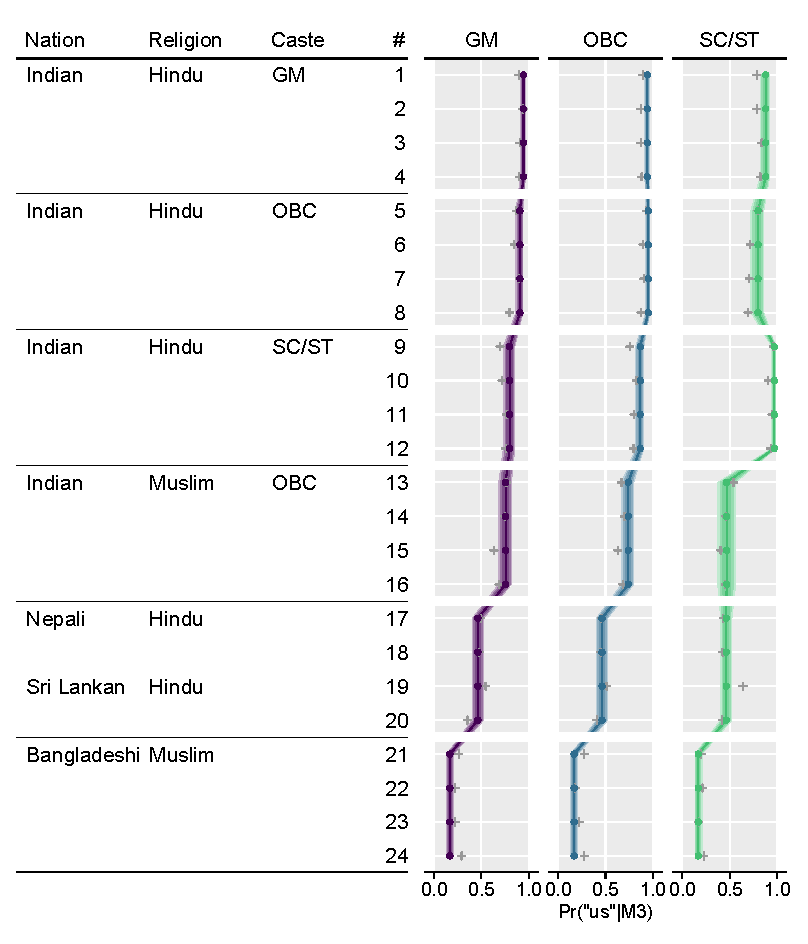
\includegraphics[scale=1]{../figures/figure-3}
\caption{
Estimated probability of participants categorizing a target as ``us'' versus ``not us'' by targets' nationality, religion, and caste (vertical), and participants' caste membership (horizontal). Dots (•) indicate the most likely \emph{estimate} for a given target's probability of being included in participants' ingroup (in Model~2, Table~\ref{tab:t2}), while the shaded ribbons encompass the 67\% (darkest shade), 89\%, and 97\% (lightest shade) most likely estimates of that probability. Pluses (+) indicate the \emph{observed} proportion of participants who included a given target in their ingroup. GM = General Merit, OBC = Other Backward Class, SC/ST = Scheduled Caste/Scheduled Tribe. % Add sentence about posterior predictive checking.
}
\label{fig:f3}
\end{figure}

\begin{figure}
\centering
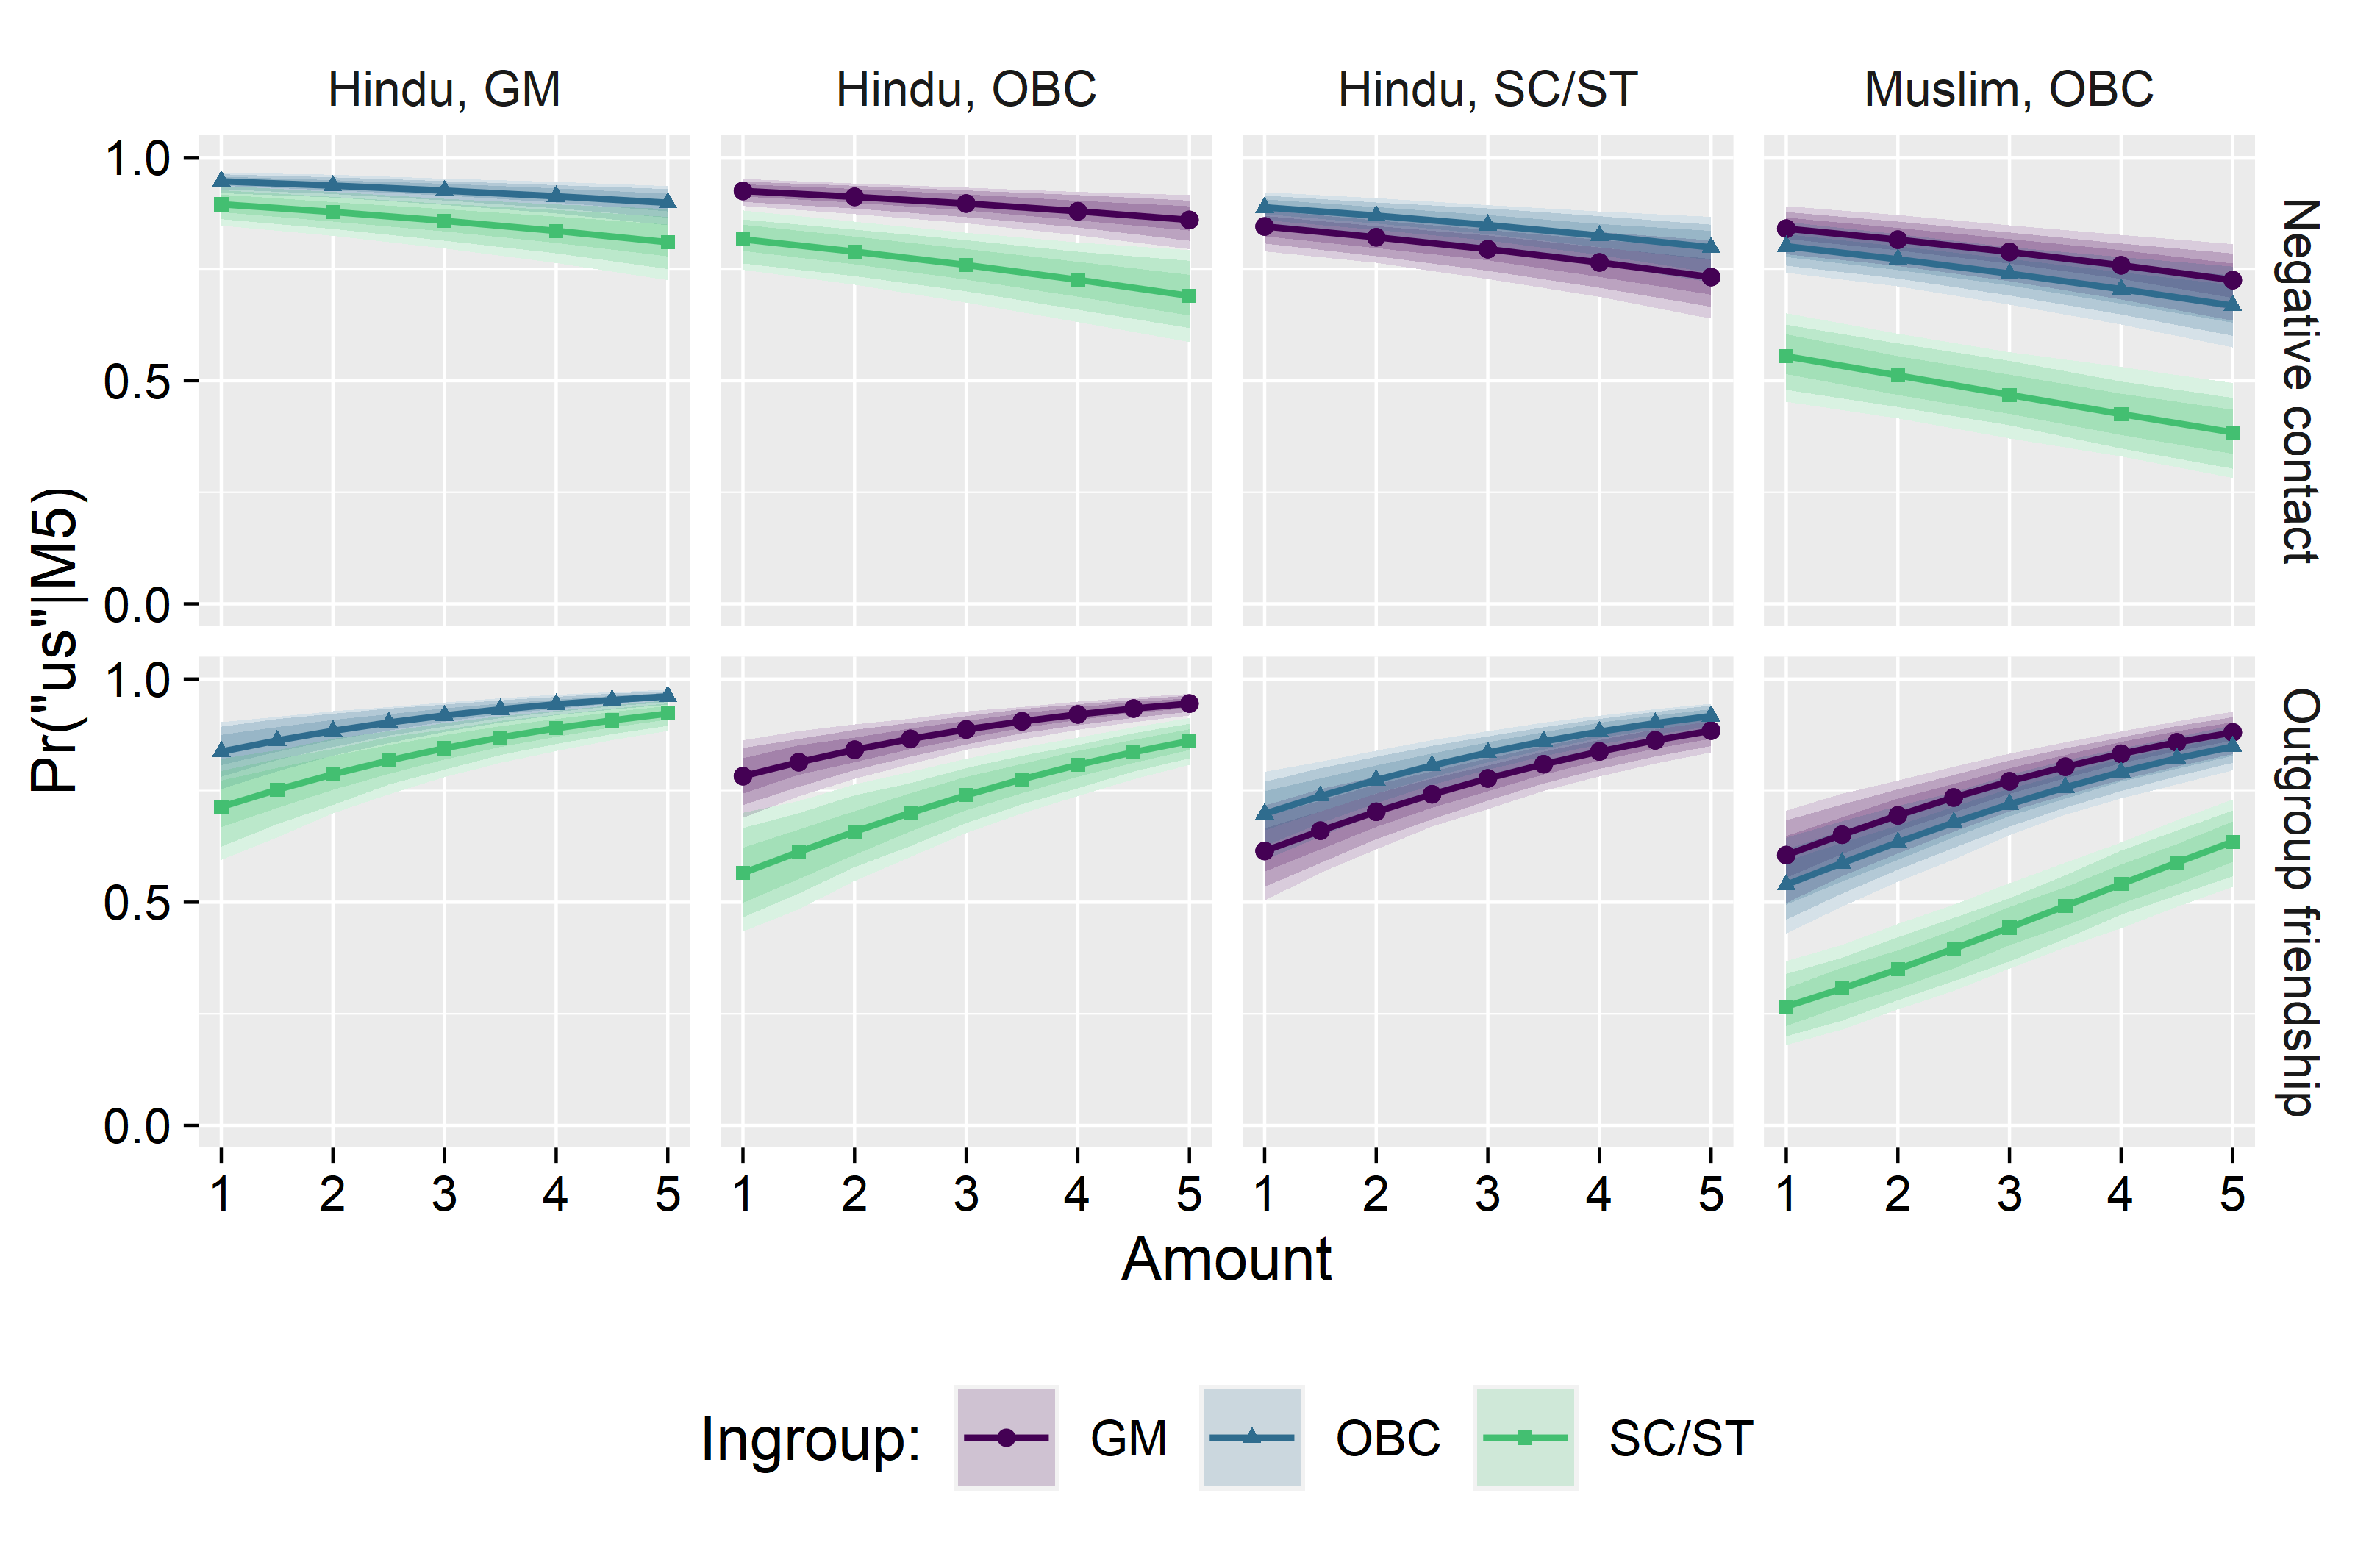
\includegraphics[scale=1]{../figures/figure-4}
\caption{Estimated probability of participants categorising a target as ``us'' versus ``not us'' as a function of the targets' group memberships (horizontal), the participants' group memberships (colour), and the reported amount of negative contact and outgroup friendship with the relevant groups (in Model~5, Table~\ref{tab:t2}). GM = General Merit, OBC = Other Backward Class, SC/ST = Scheduled Caste/Scheduled Tribe.}
\label{fig:f4}
\end{figure}

\begin{table}
\caption{Comparison of models estimating participants' social distance (SD) and feeling thermometer (FT) ratings for each target as a function of group differences and target categorizations. As in Table~\ref{tab:t2}, we selected a more complex model over a simpler model when $\frac{\Delta\textit{ELPD}}{\textit{SE}} \geq 2$. $R^2$ is a Bayesian analogue to $R^2$ in maximum likelihood estimation (Gelman, Goodrich, Gabry, \& Ali, 2017).}
\centering
\figureversion{lining, tabular}
\small	
\begin{tabularx}{\linewidth}{r@{~}rXrrrrrrr} \toprule
\# &  & Description & $R^2_\text{SD}$ & $R^2_\text{FT}$ & $\textit{ELPD}$ & $\textit{SE}$ & $\Delta\textit{ELPD}$ & $\textit{SE}$ & $\frac{\Delta\textit{ELPD}}{\textit{SE}}$ \\ \midrule 
0 &      & \ldots~(Participant) & .23 & .26 & -15203.4 & 111.8 &     - &    - &    - \\
1 & vs 0 & \ldots~(Category)    & .38 & .42 & -14300.1 & 117.9 & 903.3 & 39.6 & 22.8 \\
2 & vs 1 & \ldots~(SC/ST)       & .38 & .43 & -14248.7 & 118.2 &  51.4 &  8.8 &  5.8 \\
3 & vs 2 & \ldots~(OBC)         & .39 & .43 & -14222.2 & 118.4 &  26.5 &  7.2 &  3.7 \\ \midrule
4 & vs 3 & Categorization       & .42 & .47 & -14004.5 & 120.6 & 217.7 & 22.7 &  9.6 \\
5 & vs 4 & \ldots~(Category)    & .42 & .47 & -13986.9 & 120.9 &  17.6 &  7.7 &  2.3 \\
6 & vs 5 & \ldots~(OBC, SC/ST)  & .42 & .47 & -13988.9 & 120.8 &  -2.0 &  3.6 & -0.6 \\
\bottomrule    
\end{tabularx}
\label{tab:t3}
\end{table}

\begin{figure}
\centering
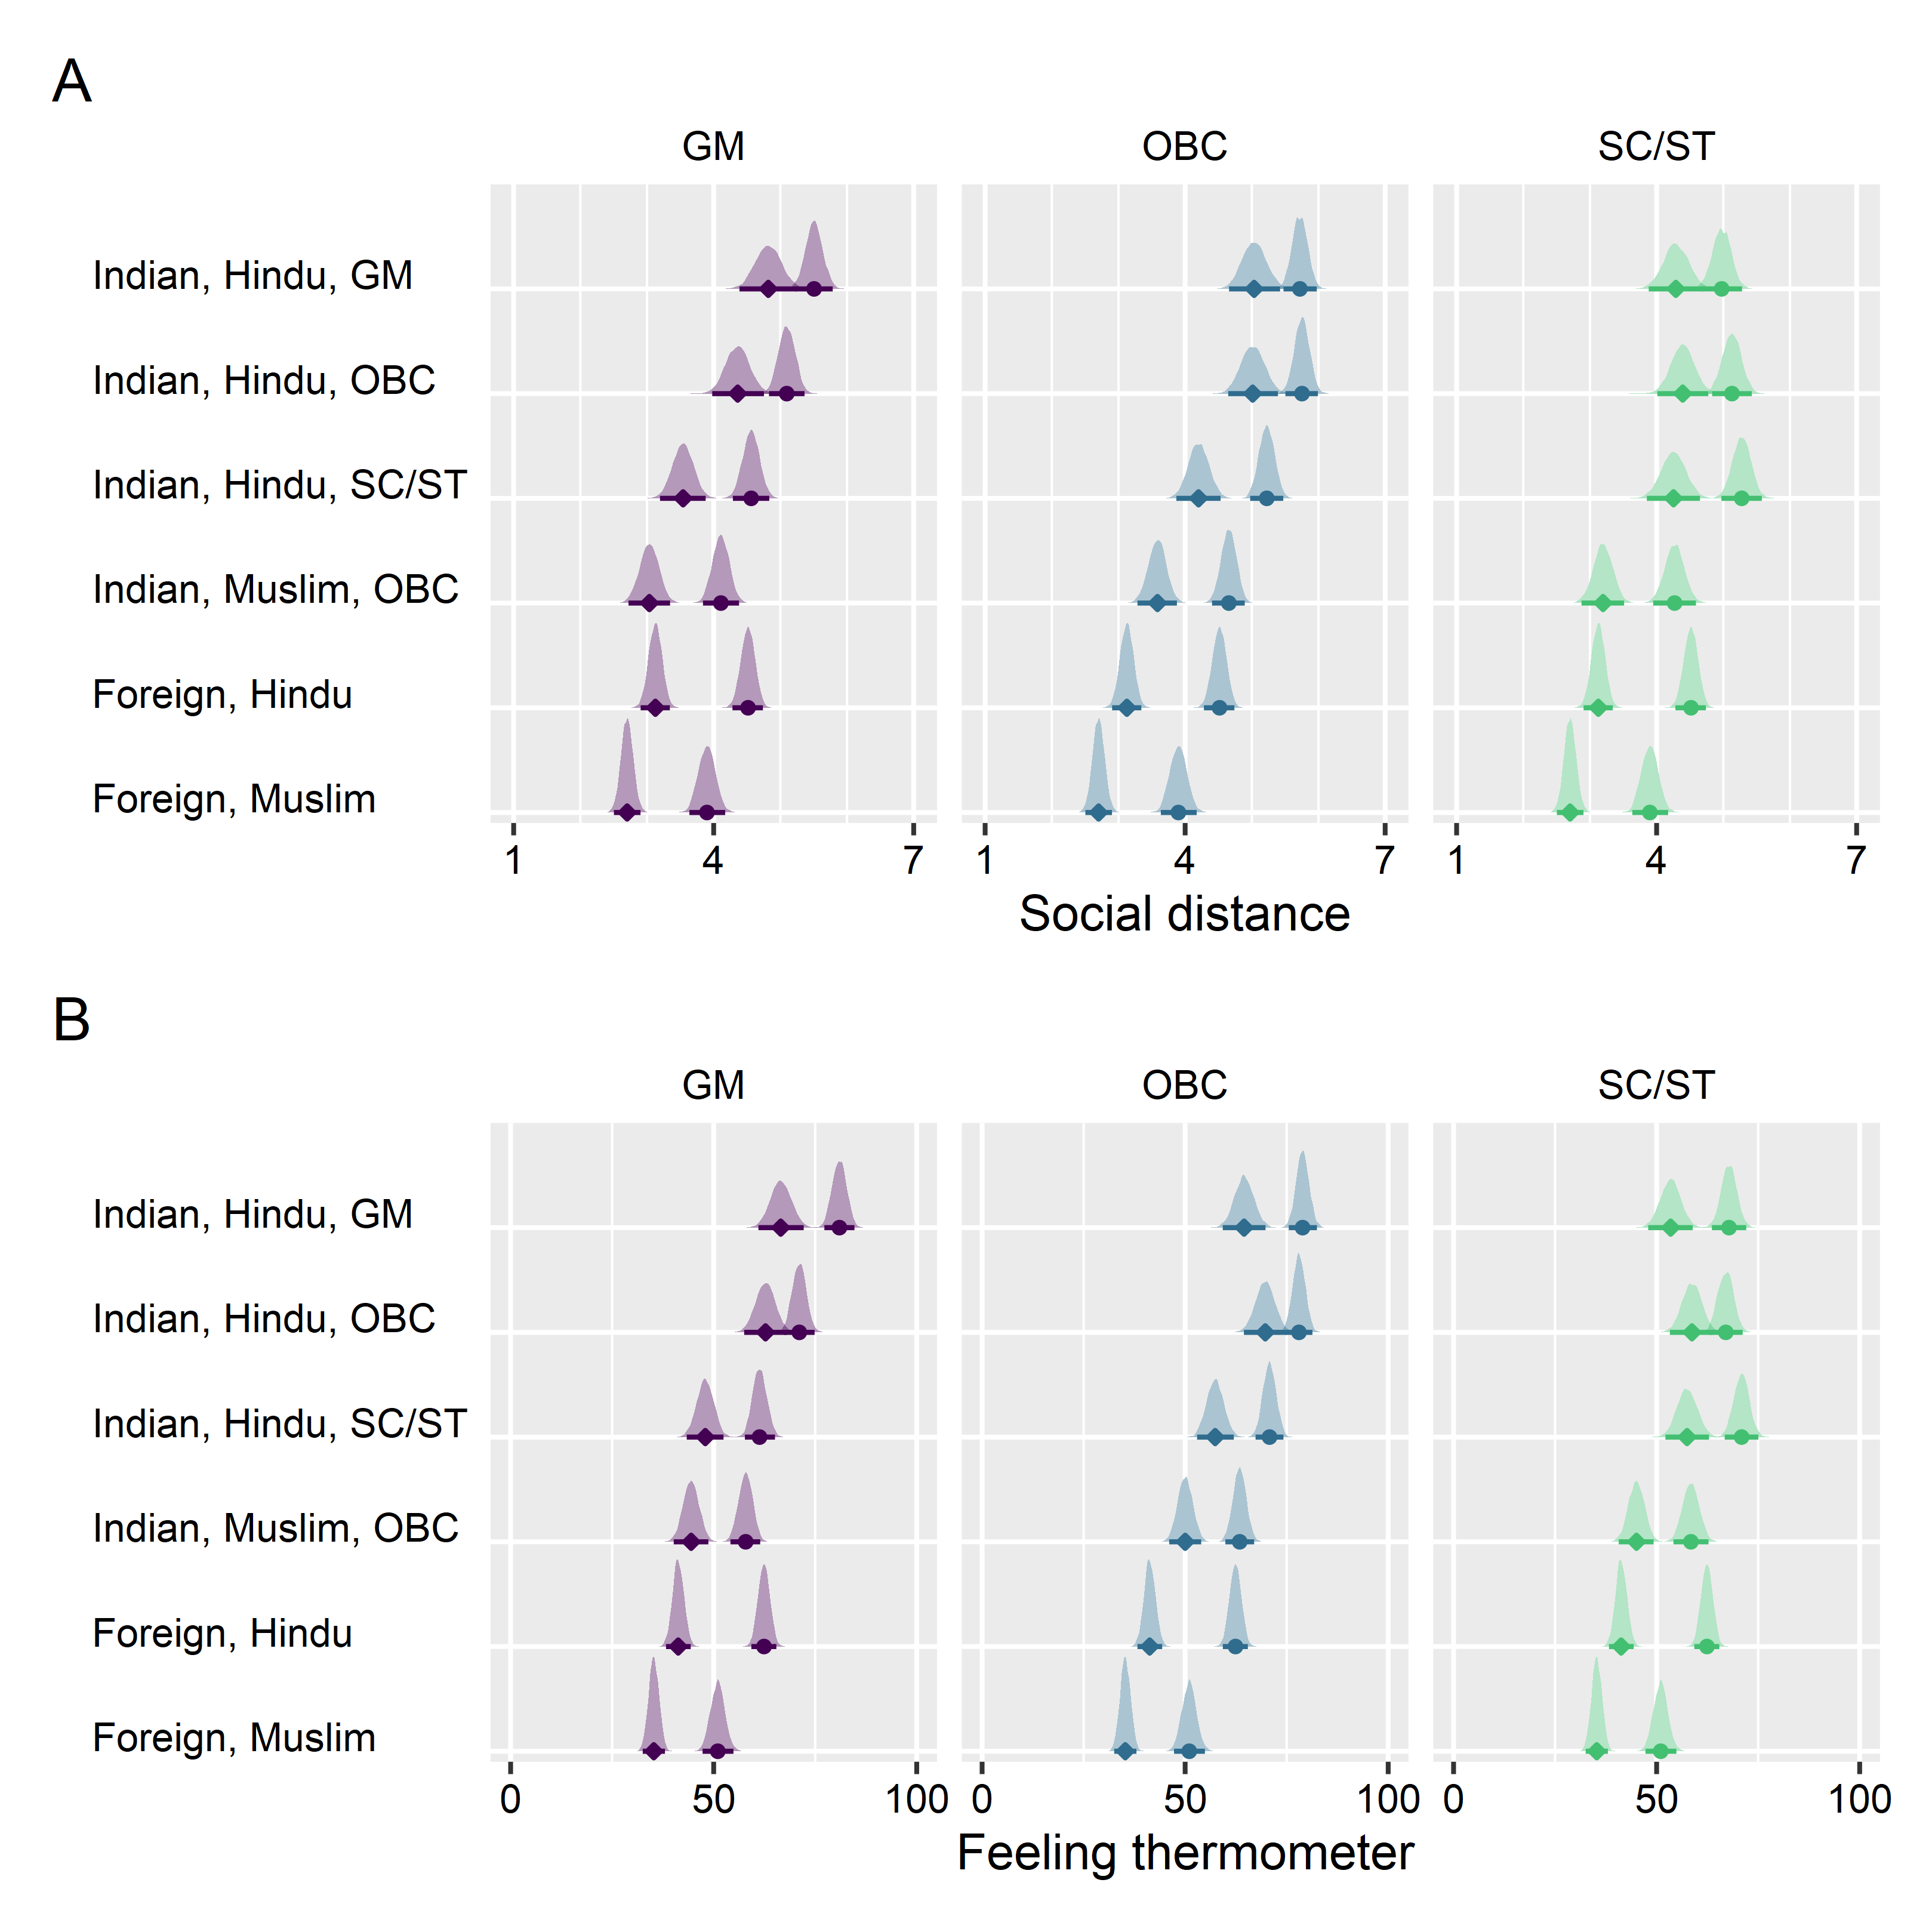
\includegraphics[scale=1]{../figures/figure-5}
\caption{
Posterior probabilities of social distance ratings as a function of target categorizations (in Model 5, Table~\ref{tab:t3}). Points are the estimated mean ratings for targets categorized as ``us''; triangles are the estimated mean ratings for targets categorized as ``not us''. GM = General Merit, OBC = Other Backward Class, SC/ST = Scheduled Caste/Scheduled Tribe.
}
\label{fig:f5}
\end{figure}

\begin{figure}
\centering
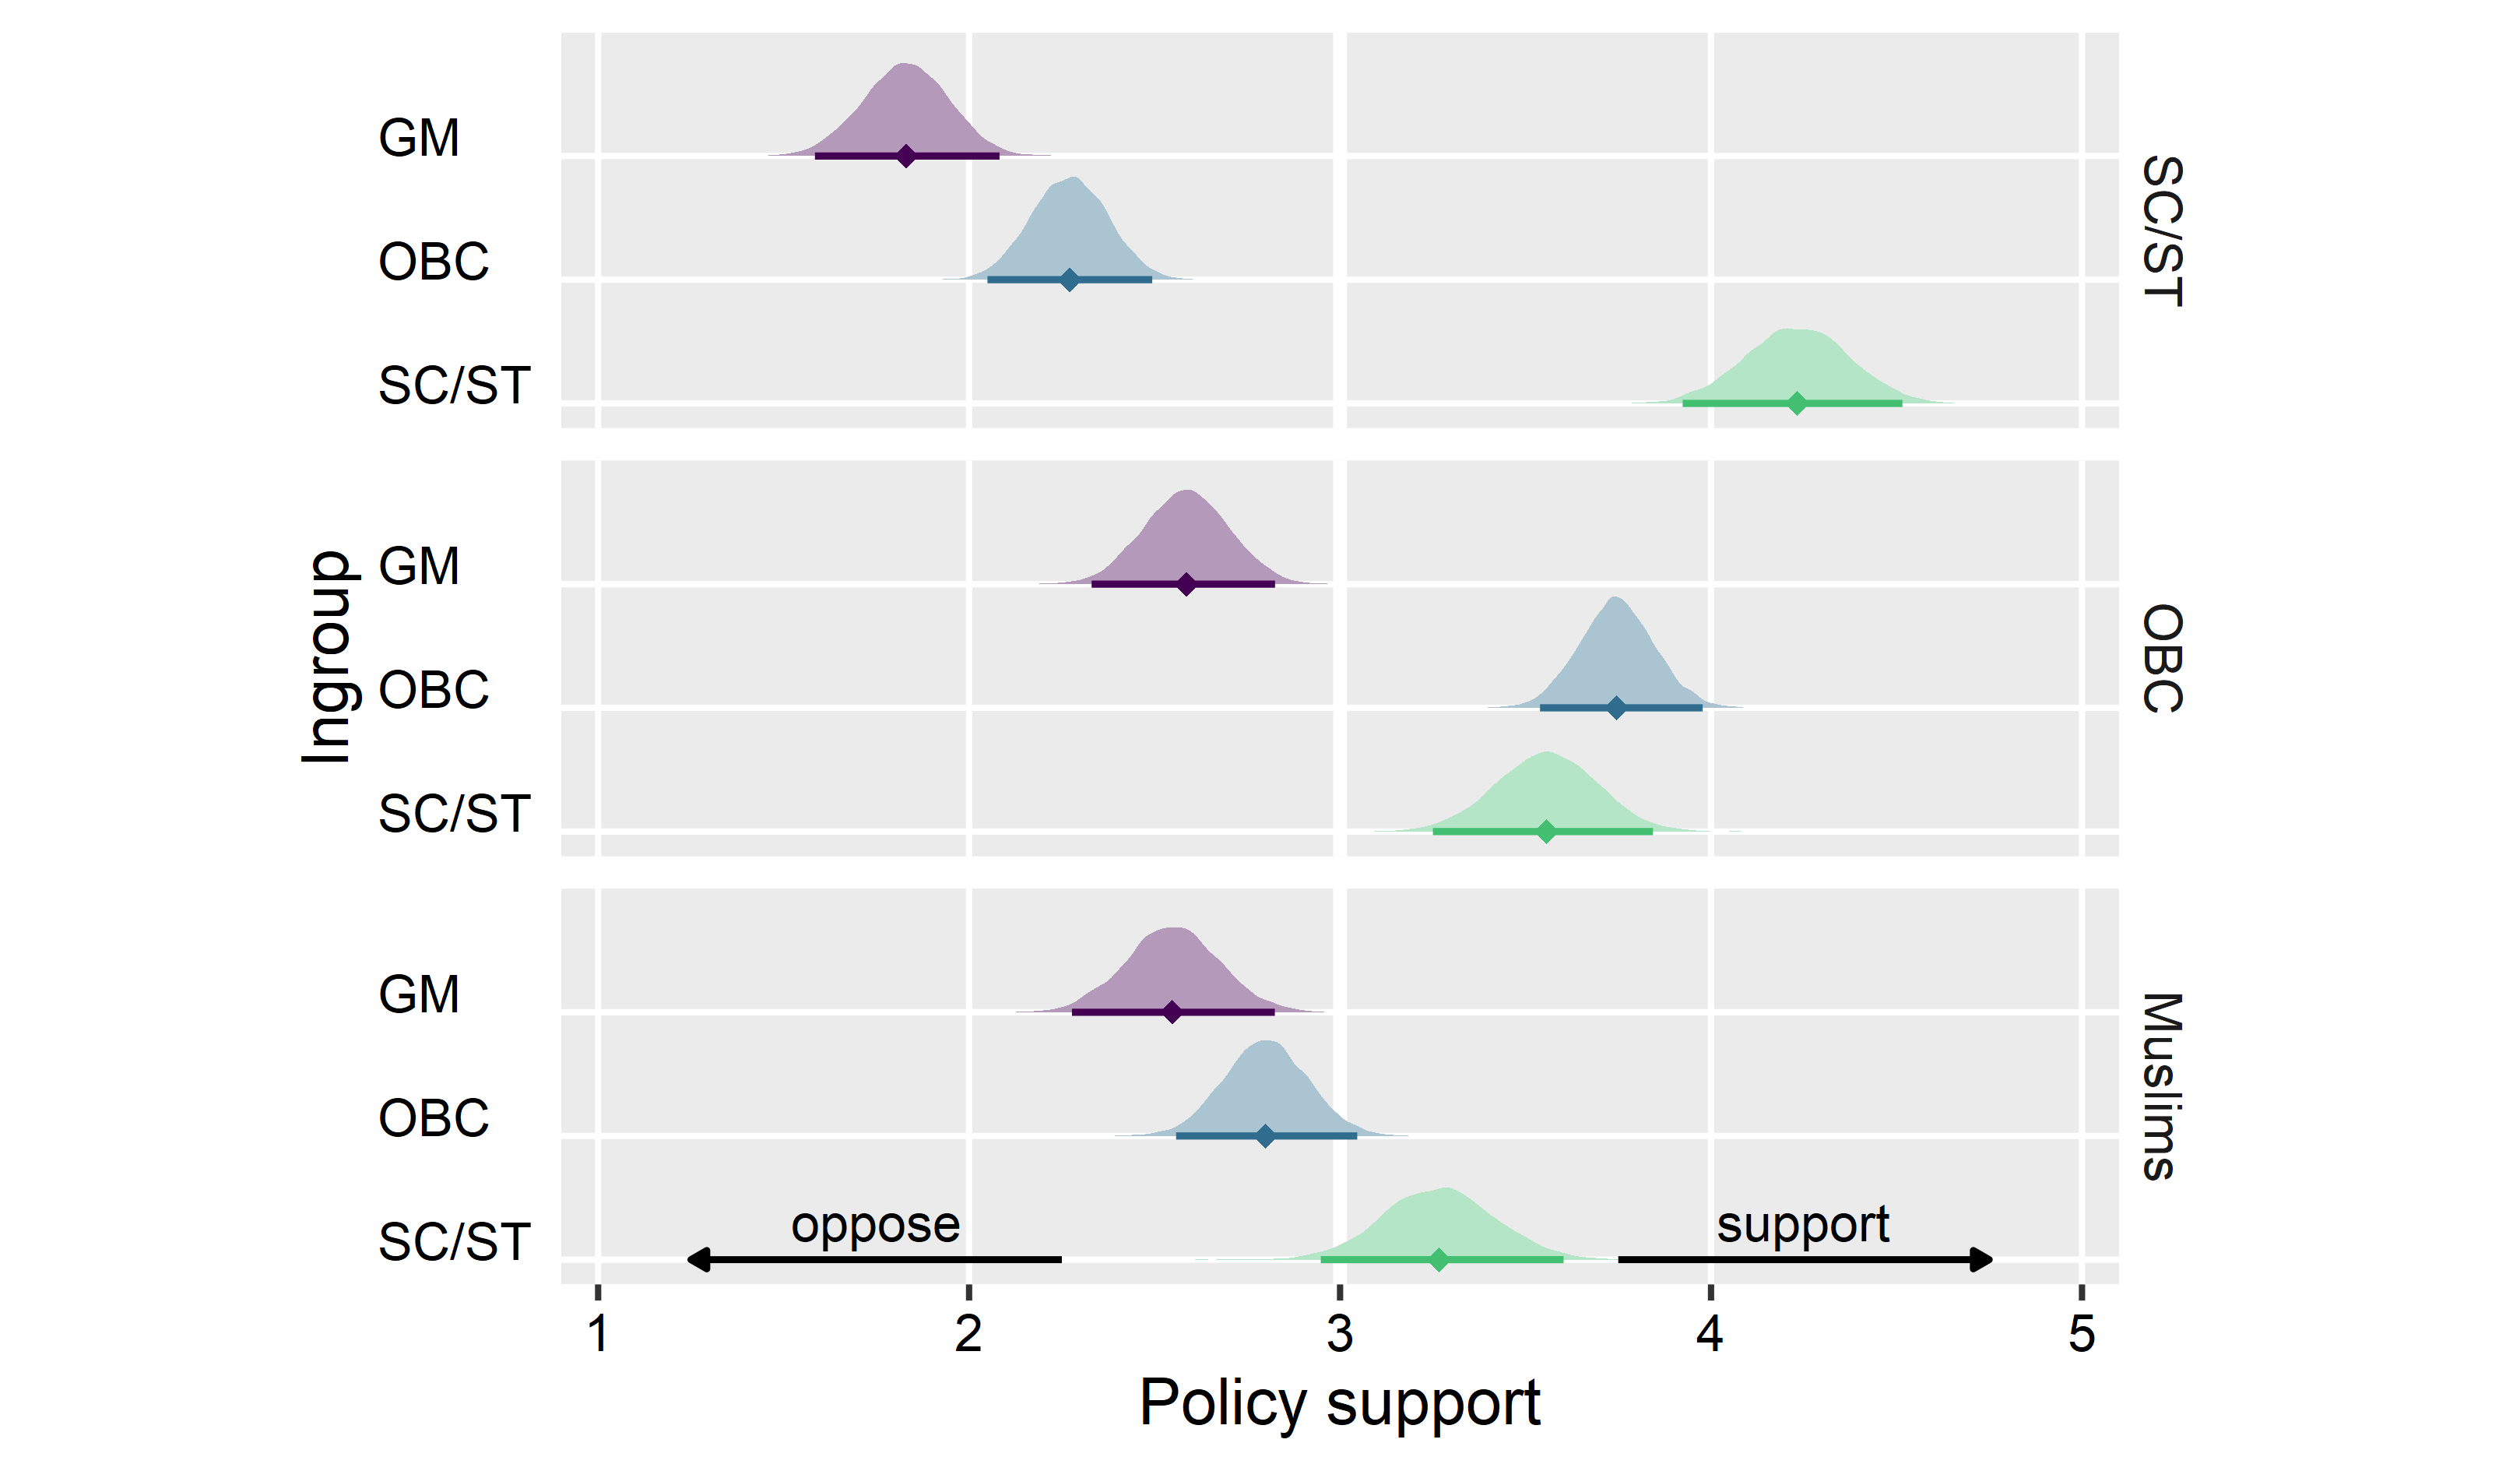
\includegraphics[scale=1]{../figures/figure-6}
\caption{
Posterior probabilities of feeling thermometer ratings as a function of target categorizations (in Model 5, Table~\ref{tab:t3}). Points are the estimated mean ratings for targets categorized as ``us''; triangles are the estimated mean ratings for targets categorized as ``not us''. GM = General Merit, OBC = Other Backward Class, SC/ST = Scheduled Caste/Scheduled Tribe.
}
\label{fig:f6}
\end{figure}

\begin{figure}
\centering
%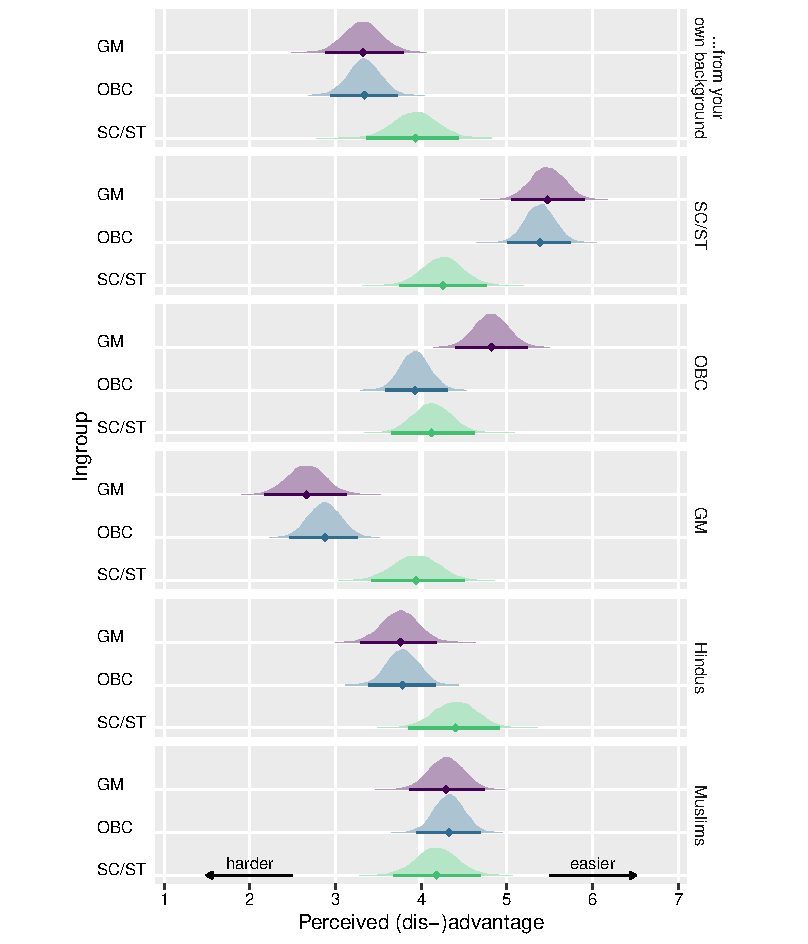
\includegraphics[scale=1]{../figures/figure-7}
\caption{\ldots GM = General Merit, OBC = Other Backward Class, SC/ST = Scheduled Caste/Scheduled Tribe.}
\label{fig:f7}
\end{figure}

\begin{figure}
\centering
%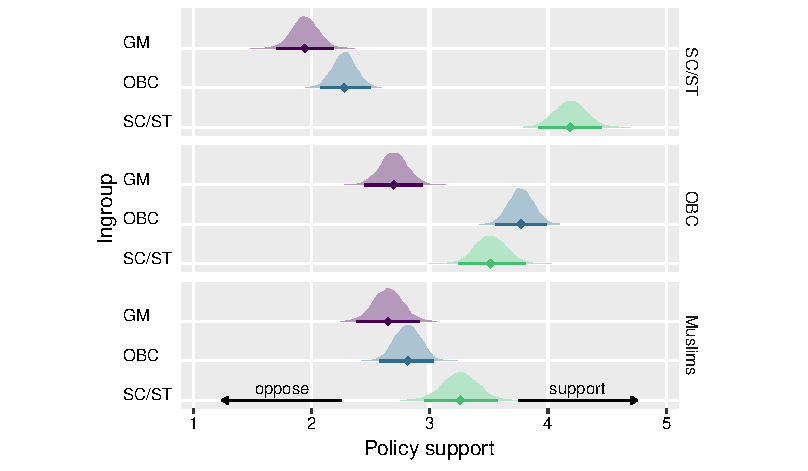
\includegraphics[scale=1]{../figures/figure-8}
\caption{\ldots GM = General Merit, OBC = Other Backward Class, SC/ST = Scheduled Caste/Scheduled Tribe.}
\label{fig:f8}
\end{figure}

\section{Discussion}

\end{document}